\chapter{Implementation and testing}
\lettrine[lines=3]{T}{} he last part of this document will describe the implementation process of the application we are developing. In the first paragraph
we will specify our development environment: Hardware, systems, developing tools and frame works, the second paragraph will be reserved for the application's
screen shots
\section{Hardware environment}
\begin{wrapfigure}[4]{r}{3cm}
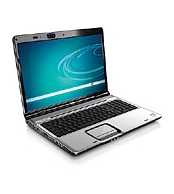
\includegraphics[width=4cm]{./images/implementation/me}
\end{wrapfigure}
\textbf{Server:} 
HP Pavilion dv9865ek Entertainment Notebook PC\newline
Intel core 2 Duo processor T8300\newline
2.4 GHZ, level 2 cache 3 MB\newline
3072 MB (1 X 1024 MB + 1 X 2048)\newline
500 GB (2X250 GB) SATA Hard Disk Drive 5400 rpm\\
\newpage
\begin{wrapfigure}[4]{r}{3cm}
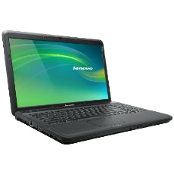
\includegraphics[width=4cm]{./images/implementation/you}
\end{wrapfigure}

\textbf{Client:}
 LENOVO G550 NTD8FFR\newline
 Intel core 2 Duo processor T6570\newline
 2.10 GHZ, level 2 cache 3 MB\newline
 3072 MB (1 X 1024 MB + 1 X 2048)\newline
 320 GB  SATA Hard Disk Drive 5400 rpm\newline
\section{Operating system}
This application was developed on Gnu/Linux system and it will be run in the mobile operating system called Android.


\section{Developing Tools}
\subsection{Eclipse}
\begin{wrapfigure}[4]{r}{3cm}

\includegraphics[width=4cm]{./images/implementation/Eclipselogo}
\end{wrapfigure}
\paragraph{Eclipse}is an integrated development environment free extensible, universal and versatile,allowing to create development projects implementing any programming language.
IDE Eclipse is written mainly in Java (using the graphics library SWT, IBM), and this language, through specific library, is also used to write extensions.
\paragraph{}The specification of Eclipse comes from the fact of its architecture fully developed around the concept of plug-in (in accordance with the OSGi standard):
the functionality of this software workshop are developed as plug-in.
\paragraph{}Several commercial software are based on free software, such as IBM Lotus Notes 8, Symphony or IBM WebSphere Studio Application Developer.
\paragraph{}This integrated development environment is a freeware set of tools to develop software in one (or more) language (s) programming. Eclipse is:
\begin{itemize}
 \item \textbf{A specialized text editor}(with syntax highlighting, automatic indentation, auto completion, ...),
 \item \textbf{A compiler}(or at least the integration of an existing compiler),
 \item \textbf{A debugger}(or at least the integration of an existing debugger)
 \item \textbf{A set of tools}for automating the compilation and management projects,
\end{itemize}
\subsection{StarUML:}
\begin{wrapfigure}[4]{r}{3cm}

\includegraphics[width=4cm]{./images/implementation/StarUML}
\end{wrapfigure}
\paragraph{}was an open source UML tool, licensed under a modified version of GNU GPL. After being abandoned for some time, 
the project had a last revival to move from Delphi to Java/Eclipse and stop again. However, 
the community is still active and many topics are discussed on the forums.\par
\paragraph{}The stated goal of the project was to replace larger, commercial applications such as Rational Rose and Borland's Together.\par
\paragraph{}StarUML supports most of the diagram types specified in UML 2.0. It is currently missing object, package, 
timing and interaction overview diagrams (though the first two can be adequately modeled through the class diagram editor).\par

\paragraph{} StarUML was written in Delphi, which is one of the reasons[1] why it was abandoned for a long time.\par

\subsection{Gimp}
\begin{wrapfigure}[4]{r}{3cm}

\includegraphics[width=4cm]{./images/implementation/gimp}
\end{wrapfigure}
\paragraph{Gimp}
is a free and open source software raster graphics editor. It is primarily employed as an image retouching and editing tool
and is freely available in versions tailored for most popular operating systems including Microsoft Windows, Apple Mac OS X, and Linux.\par
\paragraph{}
In addition to detailed image retouching and free-form drawing, GIMP can accomplish essential image editing tasks such as resizing,
 editing, and cropping photos, photomontages combining multiple images, and converting between different image formats.
 GIMP can also be used to create animated images in many formats such as GIF and MPEG through the Animation Plugin.\par
\paragraph{}
GIMP's product vision is that GIMP is a free software high-end graphics application for the editing and creation of original images, icons, graphical elements of web pages and art for user interface elements.
\subsection{Latex}
\begin{wrapfigure}[4]{l}{4cm}

\includegraphics[width=4cm]{./images/implementation/latex}
\end{wrapfigure}
\paragraph{Latex: } is a document markup language and document preparation system for the TeX typesetting program. 
Within the typesetting system, its name is styled as LaTeX. The term LaTeX refers only to the language in which documents are written, 
not to the editor used to write those documents. In order to create a document in LaTeX, a .tex file must be created using some form of text editor. 
While most text editors can be used to create a LaTeX document, 
a number of editors have been created specifically for working with LaTeX.\par 
\paragraph{}As it is distributed under the terms of the LaTeX Project Public License (LPPL), LaTeX is free software.\par
\subsection{JSON}
\begin{wrapfigure}[4]{l}{4cm}

\includegraphics[width=4cm]{./images/implementation/json}
\end{wrapfigure}
\paragraph{JSON: }(Java Object Notation) is a lightweight text-based open standard designed for human-readable data interchange.
 It is derived from the JavaScript scripting language for representing simple data structures and associative arrays, 
called objects. Despite its relationship to JavaScript, it is language-independent, with parsers available for many languages.\par

\paragraph{}The JSON format was originally specified by Douglas Crockford, and is described in RFC 4627. 
The official Internet media type for JSON is application/json. The JSON filename extension is \textbf{.json}.
\paragraph{}The JSON format is often used for serializing and transmitting structured data over a network connection.
 It is used primarily to transmit data between a server and web application, serving as an alternative to XML.\par
\subsection{JAVA}
\begin{wrapfigure}[5]{l}{4cm}

\includegraphics[width=4cm]{./images/implementation/java}
\end{wrapfigure}
\paragraph{JAVA: }Java is a programming language originally developed by James Gosling at Sun Microsystems 
(which has since merged into Oracle Corporation) and released in 1995 as a core component of Sun Microsystems' Java platform.
The language derives much of its syntax from C and C++ but has a simpler object model and fewer low-level facilities. Java applications are typically 
compiled to bytecode (class file) that can run on any Java Virtual Machine (JVM) regardless of computer architecture.\par
\paragraph{}The original and reference implementation Java compilers, virtual machines, and class libraries were developed by Sun from 1995. As of May 2007, 
in compliance with the specifications of the Java Community Process, 
Sun relicensed most of its Java technologies under the GNU General Public License. 
Others have also developed alternative implementations of these Sun technologies, such as the GNU Compiler for Java and GNU Classpath.\par
\section{realization: }
\paragraph{} The result of our application is the different interfaces to present to users.
The application is a downloadable and can be installed on different mobile devices that work
on Android operating systems.

\begin{figure}[!h]
 \center
 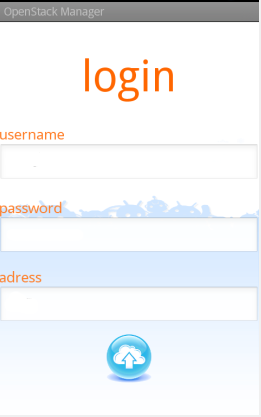
\includegraphics[width=6cm, height=8cm]{./images/implementation/login}
 \caption{connection interface}
\end{figure}
\paragraph{}This interface is the first interface that appears to the user as soon as he starts the application. 
This interface is the connection interface where the user puts his his login, 
password and address cloud.

\begin{figure}[!h]
 \center
 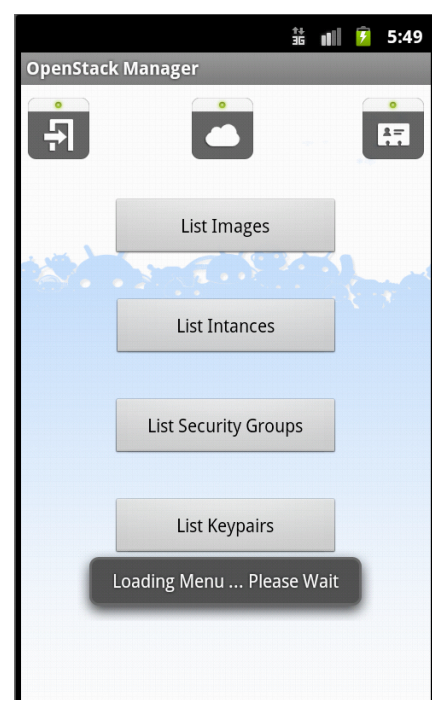
\includegraphics[width=6cm, height=8cm]{./images/implementation/menu}
 \caption{Menu List}
\end{figure}
\paragraph{}
In this second capture that is the menu list. This menu contains the different list of the application of available images,  the list of instances created, 
list of security group the user belongs etc...


\begin{figure}[!h]
 \center
 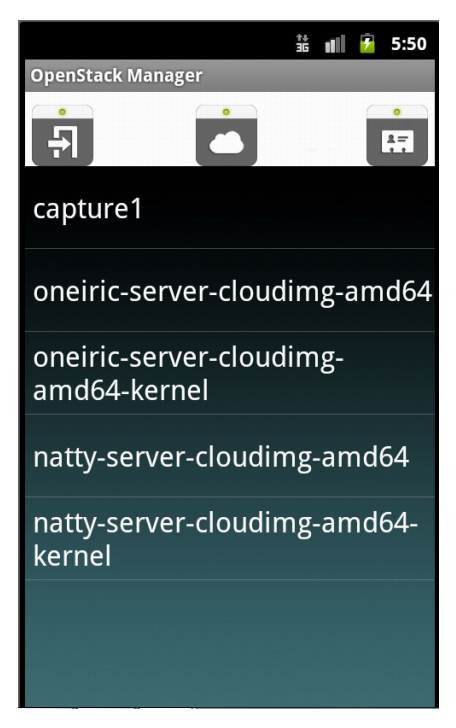
\includegraphics[width=6cm, height=8cm]{./images/implementation/images}
 \caption{Menu List}
\end{figure}
\paragraph{}in this  capture we see the difference images we have in our cloud. With this different Image API, we can create an instance by the Compute API
\section{Conclusion: }
\paragraph{}In this chapter we presented the work environment and the required tools of our application.
We have also detailed the different realization steps of the project by showing the different
interfaces of our application.\par
